\chapter{Théorie des graphes et algorithmes}
\section{Parcours d'un graphe}
\subsection{Le parcours en profondeur}
La DFS ou Depth-First Search  est la méthode la plus simple pour parcourir un graphe. Elle fonctionne sur tout type de graphe, cyclique ou non,orienté ou non.

Le procédure de parcours pour la DFS n'est pas le même pour un graphe orienté et pour un graphe non orienté.

\subsubsection{DFS pour graphe non orienté}
En principe, on choisit un sommet r racine pour démarrer la recherche ou le parcours. Puis on traverse l'arête e = (r,v) qui menè vers le sommet v. En même temps on oriente e de r vers v. Maintenant, on dit que l'arête e examiné et on l'appelle arête d'un arbre.
Le sommet r est appelé père de v et on dénote r=pere(v). On continue la recherche ou le parcours.
Au sommet x, il y a deux cas:
\begin{enumerate}
	\item si tout les arêtes incident à x ont été examiné, on retourne vers le pere de x et on continue le processus sur pere(x). On dit que le sommet x est complètement examiné.
	\item s'il existe un ou plusieurs arête(s) non examiné incident à x, alors on choisit un de ces arête e = (x,y) et on l'oriente de x vers y. Maintenant cet arête est dit "a examiné". On a deux sous cas maintenant:
	\begin{enumerate}
		\item Si y n'a pas encore été visité, on travers l'arête (x,y), on visite y et le parcours continue sur y. Dans ce cas, e = (x,y) est un arête de l'arbre et pere(y) = x.
		\item Si y a été visité auparavant, on sélectionne d'autres arêtes non examiné de x. Dans ce cas, e = (x,y) est appelé arête de retour.  
	\end{enumerate} 
\end{enumerate}
A chaque fois qu'on arrive à un nouveau sommet qui n'était pas encore visité, on lui donne un numero unique. Le numero de la racine est 1.
$$DFN(x)=numero\ courant\ du\ sommet\ x$$ 

Une DFS complète stop quand on revient à la racine et on a déjà visité tout les sommets ou quand on a trouvé le sommet/arête désiré.

La DFS divise les arêtes du graphe G en arêtes d'arbre et arêtes de retour. Manifestement, les arêtes d'arbre forme un arbre étendu de G aussi connu sous le nom de arbre de la DFS. Si on inclut les orientations des arêtes de l'arbre, on obtient un arbre orienté de la DFS. 
\begin{figure}
\centering
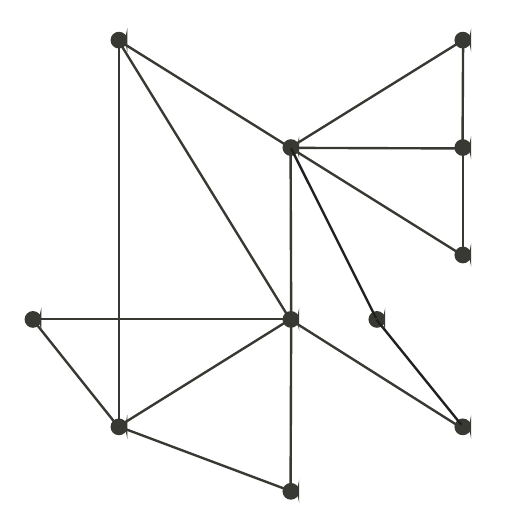
\includegraphics[width=0.3\linewidth]{images/dfs-search-example}
\caption{Graphe non-orienté: parcours DFS}
\label{fig:dfs-search-example}
\end{figure}

Pour la figure \ref{fig:dfs-search-example}, on débute la DFS sur le sommet au coin supérieur gauche.
L'arbre de la DFS correspondant est représenté par la figure 
\begin{figure}
\centering
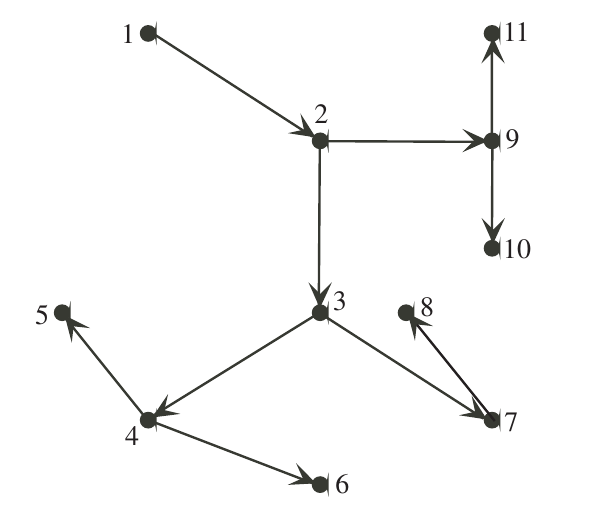
\includegraphics[width=0.3\linewidth]{images/dfs-tree-non-directed}
\caption{Arbre de la DFS correspondant au graphe non orienté \ref{fig:dfs-search-example}}
\label{fig:dfs-tree-non-directed}
\end{figure}


Dans la suite, on dénote par
\begin{equation*}
 K(x)=\left\{
 \begin{array}{l l}
 0 & \quad \text{si le sommet x n'a pas été visité}\\
 1 & \quad \text{si le sommet x a été visité}
 \end{array} \right.
\end{equation*}

et ARBRE et RETOUR sont des variables contenant les 
arêtes orientés de l'arbre et les arêtes de retour.


On peut donc représenté l'algorithme comme suit:

%\renewcommand{\algorithmicforall}{\textbf{pour tout}}
%\renewcommand{\algorithmicdo}{\textbf{faire}}
%\renewcommand{\algorithmicif}{\textbf{si}}
%\renewcommand{\algorithmicthen}{\textbf{alors}}


%\begin{algorithm}
%\caption{Depth First Search: graphe non orienté}
%\begin{algorithmic}
%\State $ARBRE \gets \emptyset$
%\State $RETOUR \gets \emptyset$
%\State $i \gets 1$
%\ForAll{sommet dans G}
%	\State $sommet.pere \gets 0$
%	\State $sommet.k \gets 0$
%\EndFor
%
%\ForAll{sommet dans G}
%	\If{ $ sommet.k = 0 $}
%		\State $i \gets i+1$
%		\State $sommet.dfn \gets i$
%		\State $sommet.k\gets 1$
%		\State $u \gets sommet$
%		\ForAll{$arête\ non\ examiné\ incident\ à\ sommet$}
%			
%			
%			
%		\EndFor	
%	\EndIf
%\EndFor
%
%
%
%\end{algorithmic}
%\end{algorithm}

%\begin{verbatim}
%ARBRE = []
%RETOUR = []
%i = 1
%pour tout sommet de G
%	sommet.pere = 0
%	sommet.k = 0
%fin pour
%
%\end{verbatim}
\begin{enumerate}
	\item Mettre  $ARBRE \leftarrow\ \emptyset,\ RETOUR \leftarrow\ \emptyset\ et\ et\ i\leftarrow\ 1$. Pour tout sommet x de G, mettre $pere(x)\leftarrow 0$ et $k(x)\leftarrow 0$
	\item Choisir un sommet r pour lequel k(r)=0 (condition utile pour les graphes non connexes, voir étape 6). Mettre  $DFN(r) \gets i,\ k(r) \gets 1,\ u \gets r$
	\item Si tous les arêtes incident à u sont tous examiné, va vers étape 5, ou alors choisir un arête e=(u,v) qui n'a pas été examiné
	\item On oriente l'arête e de u vers v et on le marque comme examiné
	\begin{enumerate}
		\item si k(v)=0, alors on met $i \gets i+1,\ DFN(v)\gets i,\ ARBRE\gets ARBRE \cup\{e\},\ k(v)\gets 1,\ pere(v)\gets u\ et\ u\gets v$, et retourne à l'étape 3
		\item si k(v)=1, alors on met $RETOUR\gets RETOUR\cup\{e\}$, et retourne à l'étape 3
	\end{enumerate}  
	\item Si $pere(u)\neq 0$, alors $u\gets pere(u)$, et on retourne à l'étape 3
	\item (Seulement pour les graphes non connexe, pour qu'on puisse passé d'un composant à un autre.) Si il existe un sommet r tel que k(r)=0, alors $i\gets i+1$ et on retourne à l'étape 2.
	\item Stop
\end{enumerate}



\subsubsection{DFS pour les graphes orientés}
La DFS dans un digraphe G (connexe et acyclique) est similaire au cas d'un graphe non orienté. L'algorithme divise les arcs de G en quatre classes différentes. Si la recherche arrive à un arc e=(x,y) non examiné, alors les quatre classes possibles sont:
\begin{enumerate}
	\item Si y n'a pas encore été visité, alors e est un arête de l'arbre de la DFS
	\item Si y a été visité, alors il y a trois cas possible:
	\begin{enumerate}
		\item y est un descendant de x dans le sous graphe induit par un arbre de la DFS existant, alors e est un arête avant et DFN(y)>DFN(x)
		\item  x est descendant de y dans le sous graphe induit par un arbre de la DFS, alors e est un arête de retour et DFN(y)<DFN(x)
		\item x et y n'ont aucune relation par rapport à aucun arbre de la DFS existant. Alors e est un arête de travers et  DFN(y)<DFN(x).(Note: il est impossible que DFN(y)>DFN(x))
	\end{enumerate}
\end{enumerate}

Le sous graphe orienté de G induit par les arêtes de l'arbre est appelé forêt de la DFS (forêt orienté). Si DFN(y)>DFN(x) pour un arc(x,y), alors (x,y) est un arête avant ou bien arête de l'arbre de la DFS.
Durant la recherche, il est facile de différentier ces deux cas puisque (x,y) est un arête de l'arbre si y n'a pas encore été visité, et arête avant sinon. Si DFN(y)<DFN(x), alors (x,y) est un arête de retour ou bien arête de travers. Durant la recherche, il est aussi facile de distinguer les deux puisque (x,y) est un arête de travers si y est complètement analysé, et arête de retour sinon.


Dans la suite, pere, k, ARBRE et RETOUR sont définis comme précédemment. On a aussi deux nouveaux variables "AVANT" et "TRAVERS" et $$L(x)= \left\{
\begin{array}{l l}
1 & \quad \text{si le x est complètement analysé}\\
0 & \quad \text{sinon}
\end{array} \right. $$ 

On peut donc présenter l'algorithme comme suit:
\begin{enumerate}
	\item Mettre  $ARBRE \leftarrow\ \emptyset,\ RETOUR \leftarrow\ \emptyset\ et\ et\ i\leftarrow\ 1,\ AVANT\gets\emptyset,\ TRAVERS\gets\emptyset$. Pour tout sommet x de G, mettre $pere(x)\leftarrow 0$, $k(x)\leftarrow 0,\ L(x)\gets0$
	\item Choisir un sommet r pour lequel k(r)=0. Mettre  $DFN(r) \gets i,\ k(r) \gets 1,\ u \gets r$
	\item Si tous les arêtes sortant de u sont tous examiné, va vers étape 5, sinon  choisir un arête e=(u,v) qui n'a pas été examiné
	\item Marque l'arc e comme examiné
	\begin{enumerate}
		\item si k(v)=0, alors on met $i \gets i+1,\ DFN(v)\gets i,\ ARBRE\gets ARBRE \cup\{e\},\ k(v)\gets 1,\ pere(v)\gets u\ et\ u\gets v$, et retourne à l'étape 3
		\item si k(v)=1 et DFN(v)>DFN(u), alors on met $AVANT\gets AVANT\cup\{e\}$, et retourne à l'étape 3
		\item si k(v)=1 et DFN(v)<DFN(u) et L(v)=0, alors on met $RETOUR\gets RETOUR\cup\{e\}$, et retourne à l'étape 3
		\item si k(v)=1 et DFN(v)<DFN(u) et L(v)=1, alors on met $TRAVERS\gets TRAVERS\cup\{e\}$, et retourne à l'étape 3
	\end{enumerate}  
	\item Si $pere(u)\neq 0$, alors $u\gets pere(u)$, et on retourne à l'étape 3
	\item (Seulement pour les graphes non connexe, pour qu'on puisse passé d'un composant à un autre.) Si il existe un sommet r tel que k(r)=0, alors $i\gets i+1$ et on retourne à l'étape 2.
	\item Stop
\end{enumerate}















 
 